\documentclass[conference]{IEEEtran}
\usepackage{cite}
\usepackage{amsmath,amssymb,amsfonts}
\usepackage{algorithmic}
\usepackage{graphicx}
\usepackage{textcomp}
\usepackage{subcaption}
\usepackage{matlab-prettifier}
\usepackage{xcolor}
\usepackage[
backend=biber,
style=ieee,
]{biblatex}
\usepackage{listings}
\usepackage{xcolor}

\definecolor{codegreen}{rgb}{0,0.6,0}
\definecolor{codegray}{rgb}{0.5,0.5,0.5}
\definecolor{codepurple}{rgb}{0.58,0,0.82}
\definecolor{backcolour}{rgb}{0.95,0.95,0.92}

\lstdefinestyle{mystyle}{
    backgroundcolor=\color{backcolour},   
    commentstyle=\color{codegreen},
    keywordstyle=\color{magenta},
    numberstyle=\tiny\color{codegray},
    stringstyle=\color{codepurple},
    basicstyle=\ttfamily\footnotesize,
    breakatwhitespace=false,         
    breaklines=true,                 
    captionpos=b,                    
    keepspaces=true,                 
    numbers=left,                    
    numbersep=5pt,                  
    showspaces=false,                
    showstringspaces=false,
    showtabs=false,                  
    tabsize=2
}

\lstset{style=mystyle}

\addbibresource{Data_Centric_Engineering.bib} %Imports bibliography file

\begin{document}

\title{Development of a Computational Fluid Dynamics Emulator using Surrogate Modelling Techniques}

\author{\IEEEauthorblockN{Magnus Jackson}
\IEEEauthorblockA{\textit{ENGM010 Data-Centric Engineering} \\
\textit{University of Exeter}}
}

\maketitle

\section{Introduction}
Computational Fluid Dynamics (CFD) is a continuously evolving research field that allows for the determination of flow patterns, forces, and many more aspects of complex fluid flow problems. As the field is developed further through both commercial and open source codes, an increasing problem complexity can be analysed to give highly accurate results. However, as the problem domain grows, or additional flow features are incorporated, the computational demand grows significantly. This means that simulations either require a large computational resource, at a high cost, or a reduction in the accuracy or scope of the problem to be evaluated \cite{moonen_employing_2015}.

The advances in understanding of Gaussian processes has led to the development of new surrogate modelling methods, which allows for the construction of emulators. An emulator is a statistical model that uses probabilistic theory and numerical simulation data to attempt to learn a specific, unknown black box function that maps the input to the output \cite{moonen_employing_2015} \cite{ding_full-field_2023}. This could also be described as a regression problem, fitting multiple dimensions to a set of training data. As a result of this, emulators can be effectively employed to investigate a wide range of input values, based on a comparatively small number of data points.

CFD is a research area that is well applied to surrogate model methods due to its non-linear characteristics and the high computational cost associated with complex problems \cite{moonen_employing_2015}. With CFD, emulators can be constructed with just a handful of inputs and outputs, which is particularly efficient when just CFD is being used to determine one or two single value outputs, such as drag or lift. Emulators can also be constructed for vector field outputs, where it will take the independent variable of interest and the associated vector field as inputs, which allows for a wider investigation and understanding of the independent variable. However, using a high number of dimensions in training can result in a complex and time consuming process, therefore when evaluating vector fields, principal component analysis (PCA) is used to reduce the dimensions of the input \cite{ding_full-field_2023} \cite{soize_probabilistic-learning-based_2024}.

Emulators have been effectively applied to a number of numerical problems, including examples such as the non linear stochastic mechanics of a 3D MEMS device \cite{soize_probabilistic-learning-based_2024}, full fields stress analysis of a connecting rod \cite{ding_full-field_2023}, thermal block analysis in 2D \cite{kapadia_active-learning-driven_2024}, and on fluid examples such as the Von Kalman vortex street and the Saint Venant equations \cite{kapadia_active-learning-driven_2024}. This demonstrates the wide range of applications the surrogate modelling approach is capable of handling.

As a relatively new research area, the methods of implementation vary significantly. There are 'traditional' approaches that use the reduced basis coefficients to generate a map between raw input to output fields \cite{ding_full-field_2023}. This method was shown to be effective for predicting accurate values, with the added advantage of having a measure of confidence in the prediction. It was also shown to be effective for both linear and non linear systems, with its efficacy increasing with the DOFs and non linearity as the computational cost of solving these more complex systems grows massively. There have also been recently proposed active learning methods, which takes an initial coarse sample to build the model and subsequently predicts values at new parameter locations which is backed up by a separate data driven surrogate \cite{kapadia_active-learning-driven_2024}. This methods allows for the construction of a high fidelity model that supports a parametric system, which again has the advantage of reducing the computational cost of a problem.


\section{Project Overview}
This project attempts to implement surrogate modelling techniques to develop an emulator for the backwards facing step flow problem. This is a widely used bench marking test in CFD for the investigation of separation flows, seen in applications such as airfoils, engine flows, and flows around buildings \cite{chen_review_2018}. This in turn means that there is a good base understanding of the problem to compare emulator results to the widely understood characteristics of a backwards facing step flow problem.

The emulator attempts to predict the recirculation length as a ratio of the step height in response to changes in the inlet velocity and the turbulent kinetic energy intensity at the inlet. The emulator used in this project utilises Gaussian processes to achieve these predictions, which is governed by the mean, $\mu$, and by the covariance matrix, $\Sigma$. To define these values, a kernel is used which controls how the input data is read and handled by the model \cite{gortler_visual_2019}. This project uses the RBF kernel which is a very commonly used kernel and has the advantage of being easily applied to a range of problems.

\clearpage
\section{Computational Methodology}
As mentioned, this paper will investigate the recirculation length of the backwards facing step, in response to changes in inlet velocity and turbulent kinetic energy intensity. In addition to the reasons discussed for the choice of this case from a validation point of view, the simplicity of the case set up will allow for the quick generation of training data. The final reason for this choice is that a mesh independence study has been completed for this geometry, and as the focus of this paper is on the construction of the emulator, it reduces time spent on the computational set up \cite{jackson_ecmm148_2023}. Both of these reasons remove the focus from the data gathering, and allow more effort to be put into the surrogate modelling methods that form the basis of this paper.

Based on the mesh independence study, a 2D mesh of 2720 cells was used for the simulations, shown in Fig.~\ref{fig:base_mesh}. This used only hexahedral type cells with a fixed aspect ratio of 1.25, and no skewness issues.

For the boundary conditions, wall type was used for the top and bottom faces including the step, the sides used the empty type and the inlet and outlet faces were patches with initial conditions assigned to them. The initial conditions were kept the same for everything except for the inlet velocity and turbulent kinetic energy intensity. The inlet velocity was varied between $0 ms^{-1}$ and $20 ms^{-1}$, and the turbulent kinetic energy intensity was varied between $0.001 ms^{-1}$ and $0.2 ms^{-1}$.

To determine the length of the recirculation zone, the 'plot over line' function in Paraview was used. Here, the velocity in the x-direction was plotted with the y value being tuned to be just above the boundary layer cells. Using this plot, the length of the recirculation zone could be taken as the point that the x velocity switched from negative to positive. Once the recirculation zone was measured, it was divided by the step height (0.2m), as is commonplace in investigations into the backwards facing step. With all data collected, this represented the raw data to be used for the training of the emulator.

\begin{figure}
    \centering
    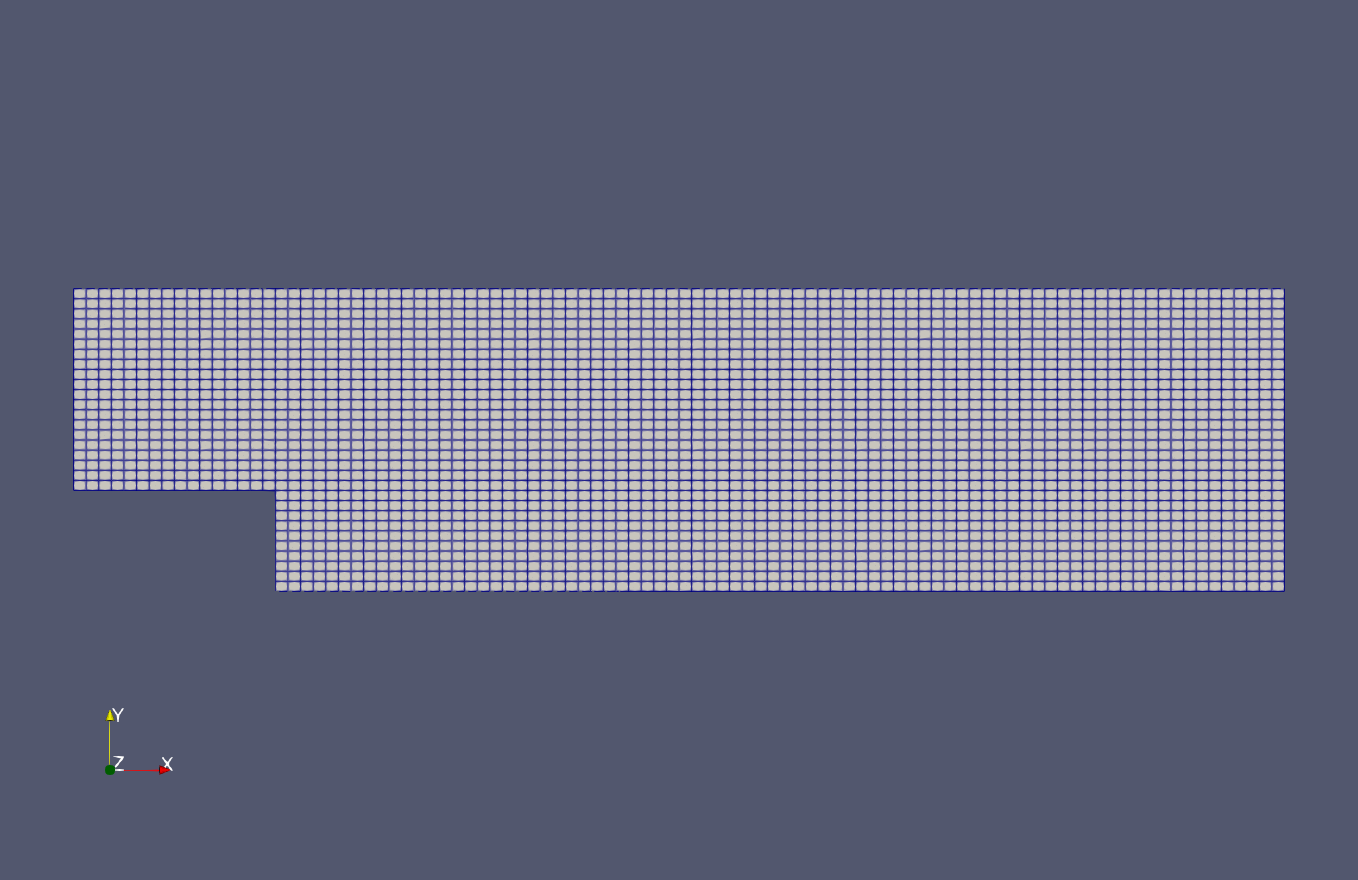
\includegraphics[width = 0.45\textwidth]{Images/base_mesh.png}
    \caption{Computational Mesh}
    \label{fig:base_mesh}
\end{figure}


\section{Surrogate Modelling Theory \& Methodology}
\subsection{Sampling}

For this paper, Latin Hypercube Sampling (LHS) was used and was implemented via the Surrogate Modelling Toolbox (SMT) in Python \cite{saves_smt_2024}. This toolbox was used as it allows for a quick and simple way to implement LHS without spending unnecessary time writing a new algorithm.

LHS is a semi random sampling method that divides the sample space into $n$ intervals in $n$ dimensions, and within each section created, a central position is assigned. The algorithm uses five main criteria to generate samples which essentially attempts to place one sample within each division of each dimension with a focus on maximising the minimum distance between points while ensuring no dimension has more than one value in each division. SMT added the fifth criteria to the framework, which uses an optimisation algorithm to enhance the results \cite{saves_smt_2024}. This method could also be described in more simple terms as a pseudo-sudoku problem. An example of the sample space LHS can generate is shown in Fig.~\ref{fig:LHS}. Careful examination of this plot shows that each sample does not have a repeated value in either dimension.

\begin{figure}
    \centering
    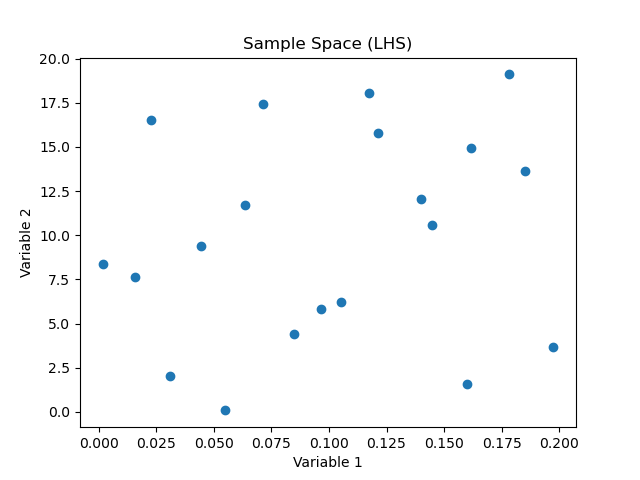
\includegraphics[width = 0.45\textwidth]{Images/lhs_example_plot.png}
    \caption{Latin Hypercube Sampling Example}
    \label{fig:LHS}
\end{figure}

\subsection{Emulator Theory \& Design}
The emulator was constructed using surrogate modelling techniques that employ Gaussian processes to generate a black box function, mapping input to output. This black box function is a multivariate Gaussian distribution over vectors of two random variables $X$ and $Y$, and the shape is governed by the mean vector $\mu$ and the covariance matrix $\Sigma$, as shown in (\ref{eq:GP}) \cite{gortler_visual_2019} . 

\begin{equation}
    P(X,Y) = \begin{bmatrix}
    X \\
    Y \\
    \end{bmatrix} \backsim \mathcal{N} (\mu,\Sigma)
    \label{eq:GP}
\end{equation}

Therefore, the emulator requires a way to covert the raw input to output into two sets of values, $\mu$ and $\Sigma$. This is done through the use of a kernel. In order to simplify the calculations, it is often assumed that $\mu = 0$, even if $\mu \neq 0$ \cite{gortler_visual_2019}. In this situation, $\mu$ is added back to the distribution after the prediction step. This process is known as centering the data.

This means that the focus is on the covariance matrix, which is determined via the kernel, $k$, or the covariance function. There are many types of kernels which can each be used for separate tasks and applications, with two main classes being stationary or non-stationary \cite{rasmussen_gaussian_2006}. For this paper, the RBF kernel will be used (2) as it is a versatile and well documented function.

\begin{equation}
    k(t,t') = \sigma^2\exp\left(-\frac{\lVert t - t' \rVert^2}{2l^2}\right)
\end{equation}

This function takes t and t' as inputs and produces a similarity measure of the two points. As a result, the entry $\Sigma_{ij}$ describes the influence that the $i$-th and $j$-th point have on each other, which in turn controls the possible shapes the fitted function can take. For the RBF kernel, the performance is controlled by the variance, $\sigma$, and the length scale, $l$, which are known as the hyperparameters. The variance determines the average distance away from the functions mean \cite{gortler_visual_2019}, while the length scale controls the reach of influence on neighbors which affects the fitting of the model to the data. Varying the length scale is the main control for under-fitting and over-fitting of the training data.

With the kernel set, the regression task can be implemented. Firstly, the raw data requires some manipulation before it can be effectively used for the training process. The input data requires normalisation to the interval $\begin{bmatrix}
    0 & 1 \\
\end{bmatrix}$ which is calculated via (3), and the output data requires standardisation to have zero mean and unit variance, calculated via (4) \cite{moonen_employing_2015}. As the data only has 2 input dimensions and 1 output dimension, there is no need to decompose the data any further.

\begin{equation}
    S[:,j] = \frac{S_{raw}[:,j]-s_{min,j}}{s_{max,j}-s_{min,j}}
\end{equation}

\begin{equation}
    Y[i,:] = \frac{Y_{raw}[i,:]-y_{avg,i}}{y_{std,i}}
\end{equation}

The posterior distribution, $P(X|Y)$, can now be obtained by observing the modified training data. The first step is to form the joint probability distribution, $P_{X,Y}$, giving a multivariate Gaussian distribution with dimensions equal to that of the test points and of the training data. Through the process of conditioning, the posterior $P(X|Y)$ can be found from $P_{X,Y}$ which produces derived versions of the mean and standard deviation \cite{gortler_visual_2019}. This results in a conditional distribution which forces the set of function to pass through the training points. Marginalisation is then used to extract the mean function value and standard deviation from each $i$-th point. This gives the final distribution to map the input to output.

The model was then improved using an acquisition function to generate the next sample point to evaluate the design space at. For this paper, an arbitrary aim was taken to minimise the recirculation length, although this method could easily be modified to maximise a value too. This function aims to select a point that will yield a good quality solution and explore areas where the uncertainty is high \cite{de_ath_what_2020}. This was used to select the initial conditions for 4 more training points to improve the model, following the initial training using the 20 data points from LHS.

To implement this process in Python, the toolbox \texttt{sciKitLearn} was used \cite{pedregosa_scikit-learn_2011}. This was used as it easily implements the kernel for Gaussian regression problems, and has the capability to tune the hyperparameters for optimal performance. In addition to this, the kernel optimisation and subsequent training can be easily controlled through keyword arguments. 


\section{Results}
\subsection{Training Data Results}
Using LHS, an initial set of 20 points was generated for simulation initial conditions. The recirculation length and associated step height ratio was found, with each member of the group doing 5 simulations each. An example of the velocity magnitude plot is shown in Fig.~\ref{fig:vmag}. The raw data initially gathered is shown in Table~\ref{tab: raw_data}.

\begin{figure}[ht]
    \centering
    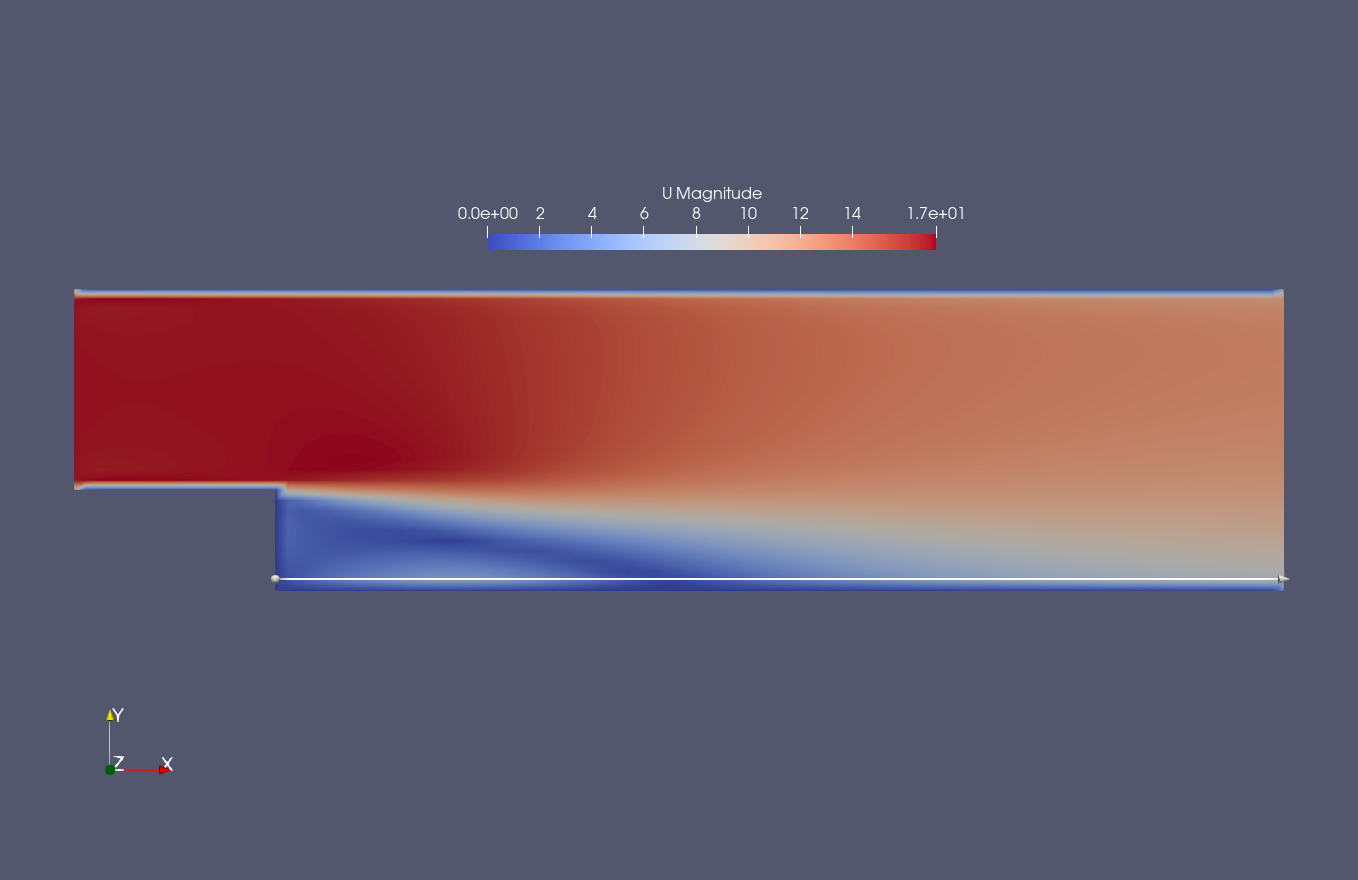
\includegraphics[width = 0.45\textwidth]{Images/result_example.png}
    \caption{Velocity Magnitude Plot}
    \label{fig:vmag}
\end{figure}

\begin{table}[ht]
\centering
\caption{Raw Data}
\begin{tabular}{|l|ll|ll|}
\hline
\multicolumn{1}{|c|}{Sample} & \multicolumn{1}{c}{k} & \multicolumn{1}{c|}{U $ms^{-1}$} & \multicolumn{1}{c}{Recirc. Length (m)} & \multicolumn{1}{c|}{Ratio of H} \\ \hline
1                            & 0.1283970                                   & 16.92780               & 0.3815                                     & 1.9075                          \\
2                            & 0.0571957                                   & 1.84931                & 0.4165                                     & 2.0825                          \\
3                            & 0.1637660                                   & 3.72207                & 0.3595                                     & 1.7975                          \\
4                            & 0.1767490                                   & 12.51520               & 0.3525                                     & 1.7625                          \\
5                            & 0.0794834                                   & 9.15597                & 0.4206                                     & 2.103                           \\
6                            & 0.0933685                                   & 4.1109                 & 0.4043                                     & 2.02134                         \\
7                            & 0.0120645                                   & 8.79247                & 0.4061                                     & 2.03035                         \\
8                            & 0.0631101                                   & 10.67490               & 0.4092                                     & 2.045915                        \\
9                            & 0.1548780                                   & 2.79451                & 0.4048                                     & 2.024165                        \\
10                           & 0.1024480                                   & 0.15698                & 0.3702                                     & 1.85084                         \\
11                           & 0.0013705                                   & 5.03365                & 0.4077                                     & 2.038455                        \\
12                           & 0.0302337                                   & 11.55950               & 0.4074                                     & 2.037135                        \\
13                           & 0.1971570                                   & 7.37160                & 0.4062                                     & 2.03079                         \\
14                           & 0.1109730                                   & 15.61010               & 0.4060                                     & 2.030245                        \\
15                           & 0.0877914                                   & 13.78100               & 0.4085                                     & 2.04263                         \\
16                           & 0.1829830                                   & 19.36090               & 0.447                                      & 2.235                           \\
17                           & 0.1403020                                   & 14.24820               & 0.439                                      & 2.195                           \\
18                           & 0.0468786                                   & 18.21260               & 0.471                                      & 2.355                           \\
19                           & 0.1379370                                   & 17.49050               & 0.448                                      & 2.24                            \\
20                           & 0.0379453                                   & 6.11915                & 0.428                                      & 2.14                            \\ \hline
\end{tabular}
\label{tab: raw_data}
\end{table}

\subsection{Emulator Results}
The initial data set from Table \ref{tab: raw_data} was used to produce Fig.~\ref{fig:recirc_orig}, \ref{fig:std_orig}, and ~\ref{fig:ei_orig}. The colour scale had to be limited in Fig.~\ref{fig:recirc_orig} due to high values in the corners, losing resolution in the middle where the main investigation was focused. Following this, the optimisation steps were carried out, generating the new points shown in Table \ref{tab:optim_values}, with results shown in Fig.~\ref{fig:recirc_optim}, \ref{fig:std_optim}, and \ref{fig:ei_optim}.

\begin{figure}[ht]
    \centering
    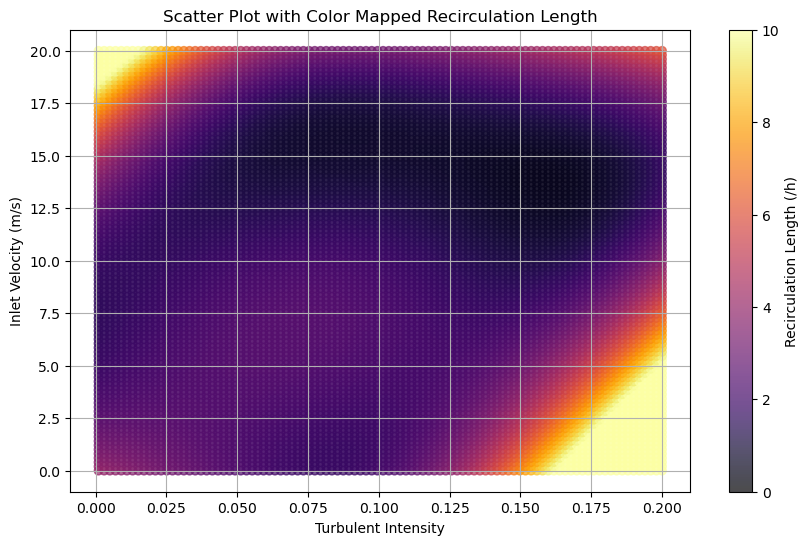
\includegraphics[width = 0.45\textwidth]{Images/recirc_orig.png}
    \caption{Initial Plot of Recirculation Length}
    \label{fig:recirc_orig}
\end{figure}
\begin{figure}[ht]
    \centering
    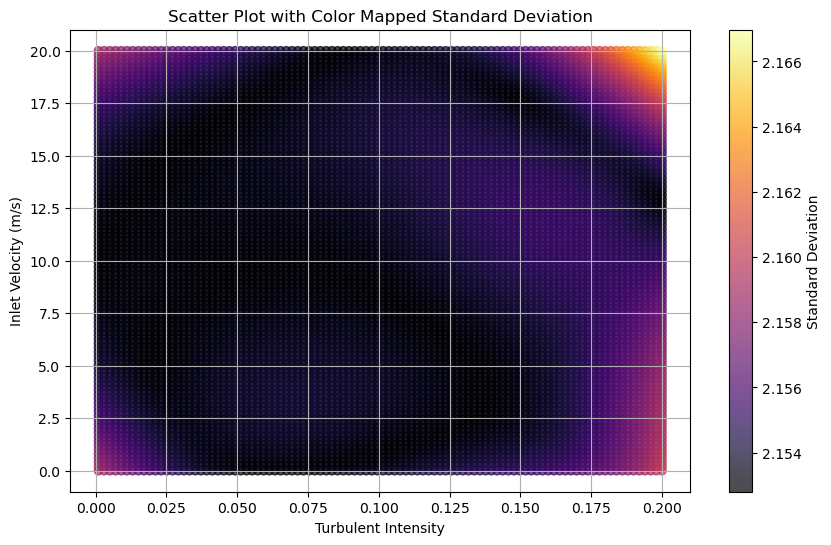
\includegraphics[width = 0.45\textwidth]{Images/std_orig.png}
    \caption{Initial Plot of Standard Deviation}
    \label{fig:std_orig}
\end{figure}
\begin{figure}[ht]
    \centering
    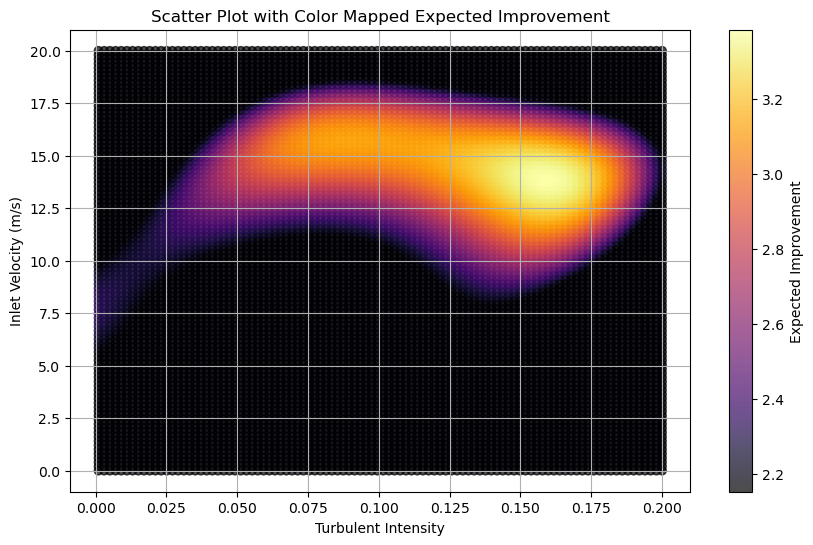
\includegraphics[width = 0.45\textwidth]{Images/ei_orig.png}
    \caption{Initial Plot of Expected Improvement}
    \label{fig:ei_orig}
\end{figure}


\begin{figure}[ht]
        \centering
        \begin{subfigure}[b]{0.39\textwidth}
            \centering
            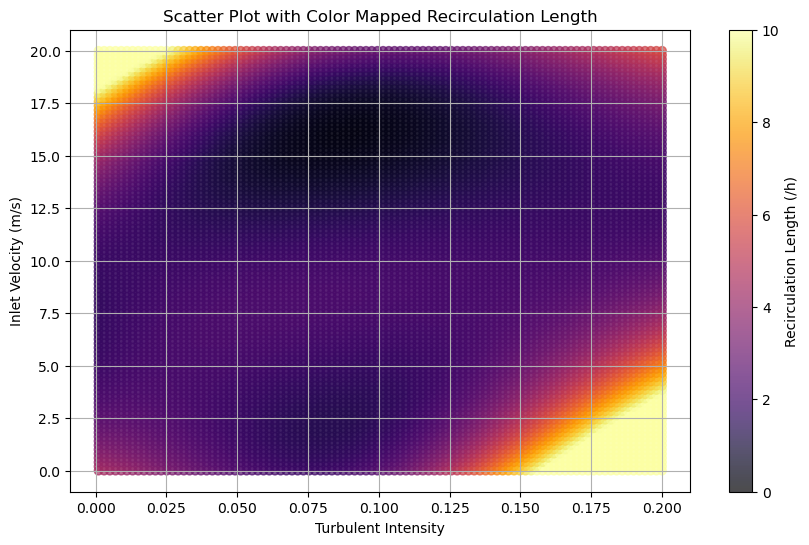
\includegraphics[width=\textwidth]{Images/recirc_1.png}
            \caption[]%
            {{\small Optimisation 1}}    
            \label{fig:recirc_1}
        \end{subfigure}
        \vskip \baselineskip
        \begin{subfigure}[b]{0.39\textwidth}  
            \centering 
            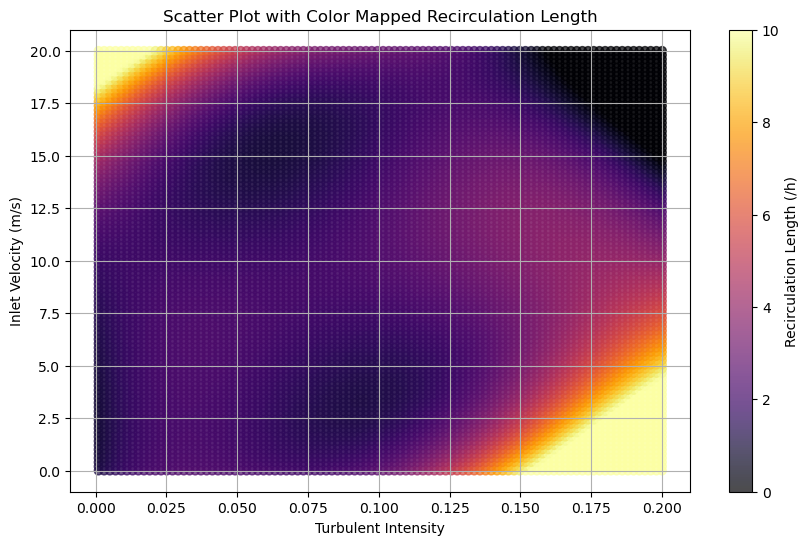
\includegraphics[width=\textwidth]{Images/recirc_2.png}
            \caption[]%
            {{\small Optimisation 2}}    
            \label{fig:recirc_2}
        \end{subfigure}
        \vskip \baselineskip
        \begin{subfigure}[b]{0.39\textwidth}
            \centering
            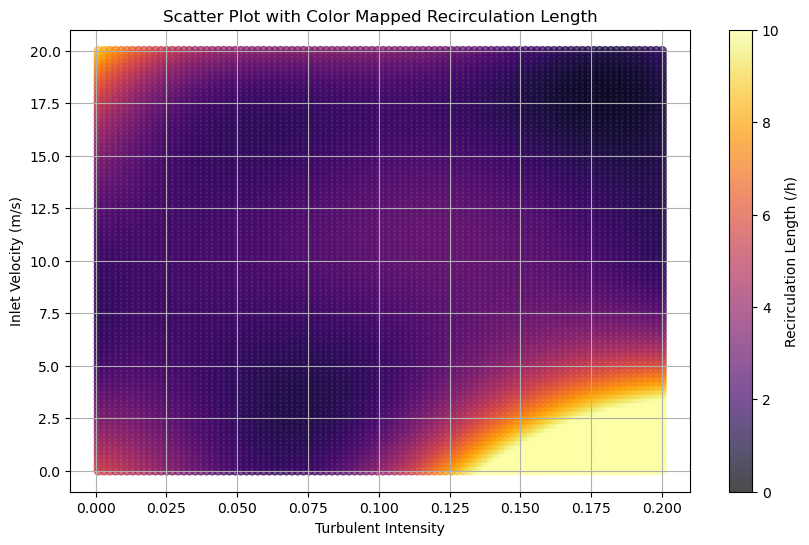
\includegraphics[width=\textwidth]{Images/recirc_3.png}
            \caption[]%
            {{\small Optimisation 3}}    
            \label{fig:recirc_3}
        \end{subfigure}
        \vskip \baselineskip
        \begin{subfigure}[b]{0.39\textwidth}  
            \centering 
            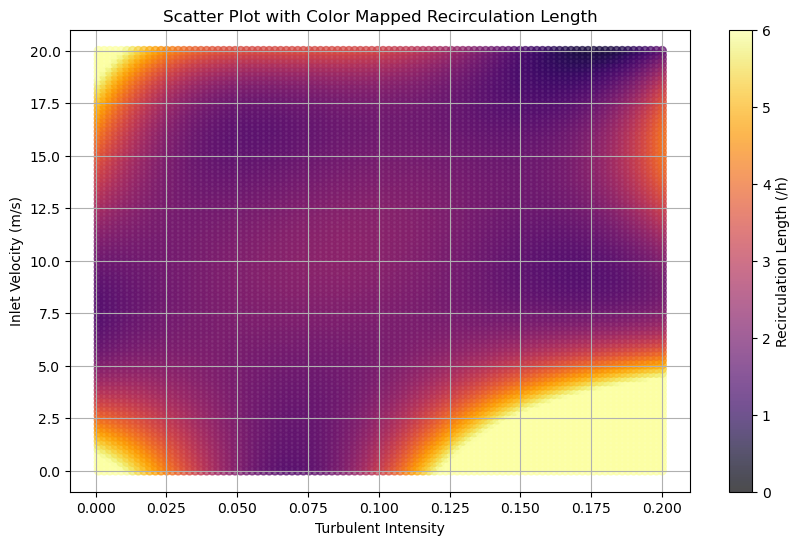
\includegraphics[width=\textwidth]{Images/recirc_4.png}
            \caption[]%
            {{\small Optimisation 4}}    
            \label{fig:recirc_4}
        \end{subfigure}
        \caption[]%
        {\small Recirculation Length Optimisation} 
        \label{fig:recirc_optim}
\end{figure}

\begin{figure}[ht]
        \centering
        \begin{subfigure}[b]{0.39\textwidth}
            \centering
            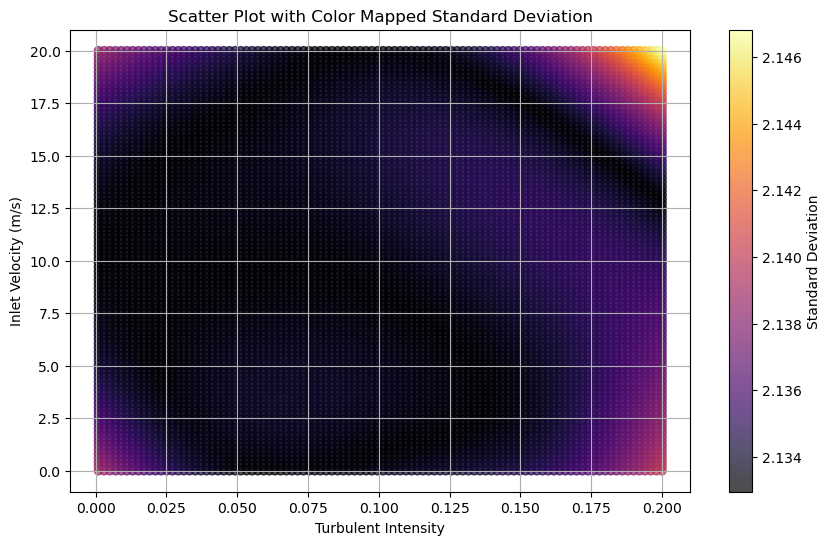
\includegraphics[width=\textwidth]{Images/std_1.png}
            \caption[]%
            {{\small Optimisation 1}}    
            \label{fig:std_1}
        \end{subfigure}
        \vskip \baselineskip
        \begin{subfigure}[b]{0.39\textwidth}  
            \centering 
            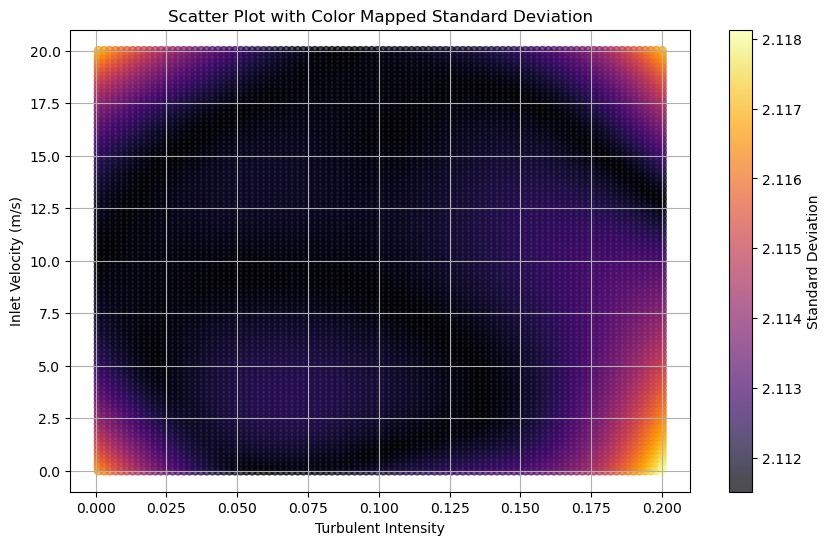
\includegraphics[width=\textwidth]{Images/std_2.png}
            \caption[]%
            {{\small Optimisation 2}}    
            \label{fig:std_2}
        \end{subfigure}
        \vskip \baselineskip
        \begin{subfigure}[b]{0.39\textwidth}
            \centering
            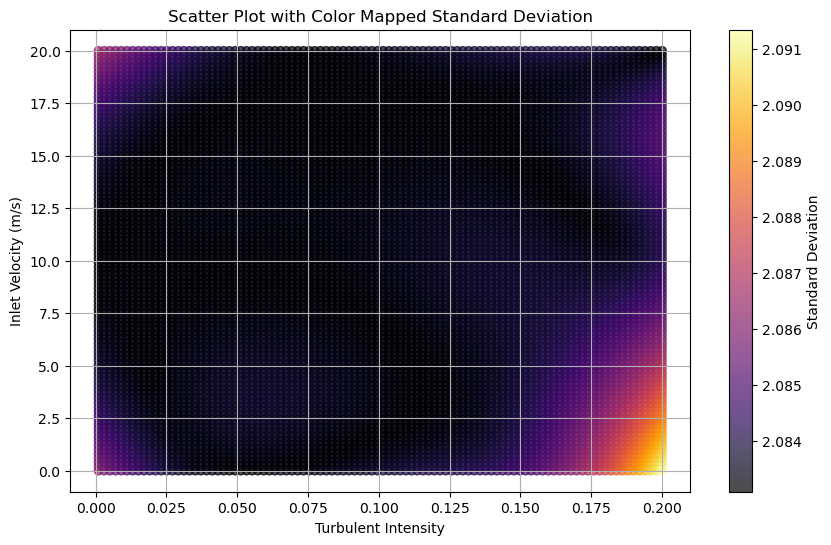
\includegraphics[width=\textwidth]{Images/std_3.png}
            \caption[]%
            {{\small Optimisation 3}}    
            \label{fig:std_3}
        \end{subfigure}
        \vskip \baselineskip
        \begin{subfigure}[b]{0.39\textwidth}  
            \centering 
            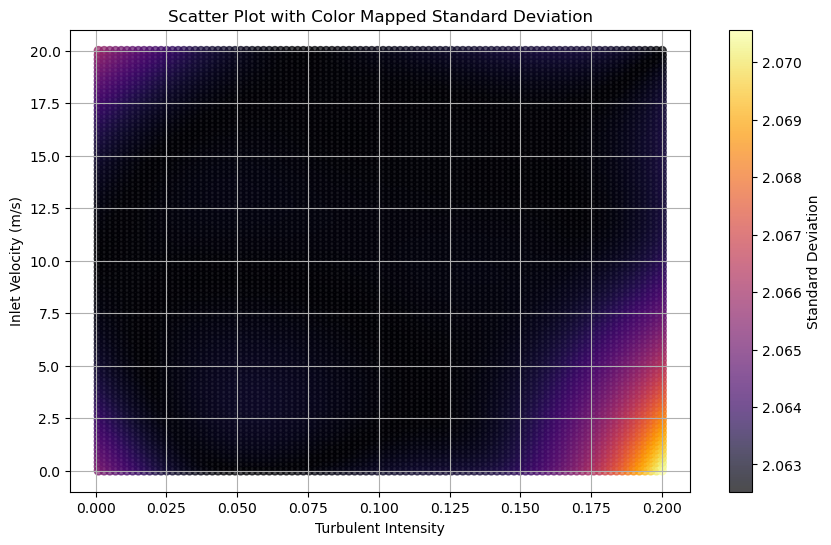
\includegraphics[width=\textwidth]{Images/std_4.png}
            \caption[]%
            {{\small Optimisation 4}}    
            \label{fig:std_4}
        \end{subfigure}
        \caption[]%
        {\small Standard Deviation Optimisation} 
        \label{fig:std_optim}
\end{figure}

\begin{figure}[ht]
        \centering
        \begin{subfigure}[b]{0.39\textwidth}
            \centering
            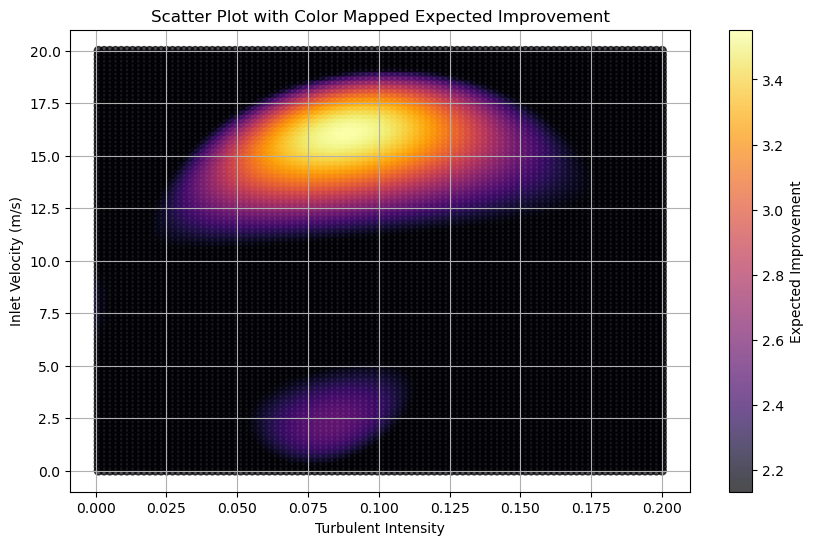
\includegraphics[width=\textwidth]{Images/ei_1.png}
            \caption[]%
            {{\small Optimisation 1}}    
            \label{fig:ei_1}
        \end{subfigure}
        \vskip \baselineskip
        \begin{subfigure}[b]{0.39\textwidth}  
            \centering 
            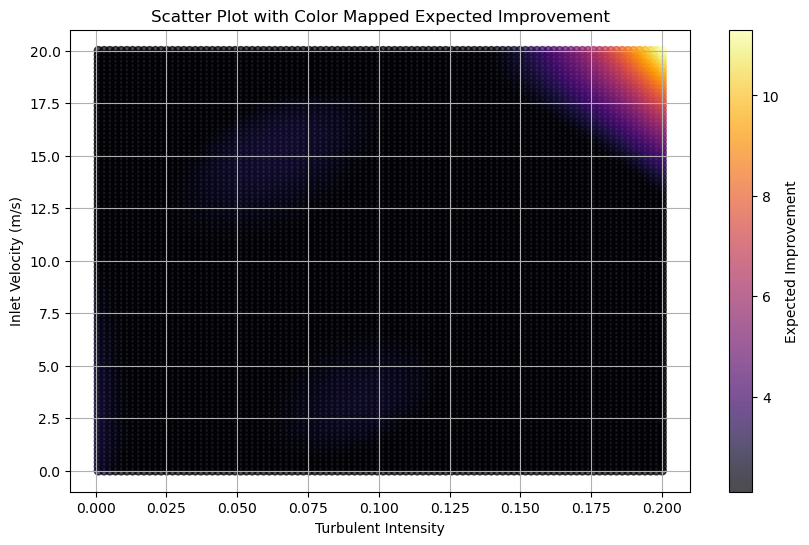
\includegraphics[width=\textwidth]{Images/ei_2.png}
            \caption[]%
            {{\small Optimisation 2}}    
            \label{fig:ei_2}
        \end{subfigure}
        \vskip \baselineskip
        \begin{subfigure}[b]{0.39\textwidth}
            \centering
            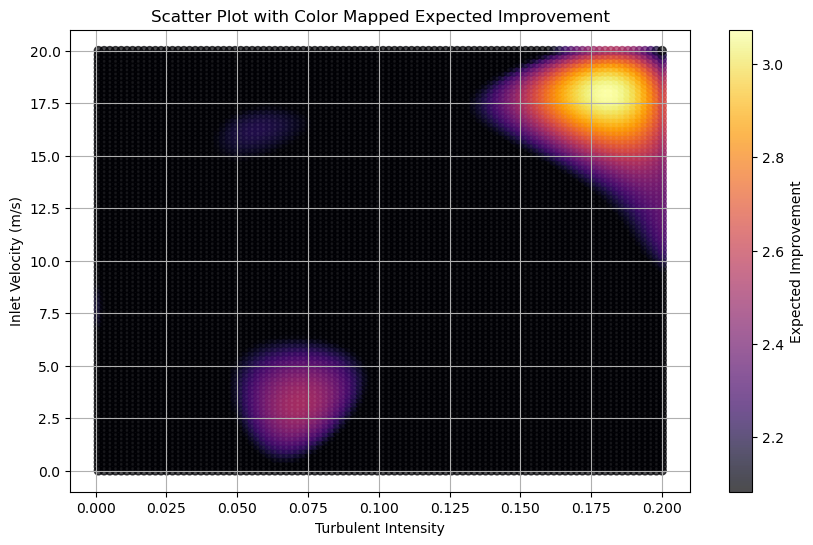
\includegraphics[width=\textwidth]{Images/ei_3.png}
            \caption[]%
            {{\small Optimisation 3}}    
            \label{fig:ei_3}
        \end{subfigure}
        \vskip \baselineskip
        \begin{subfigure}[b]{0.39\textwidth}  
            \centering 
            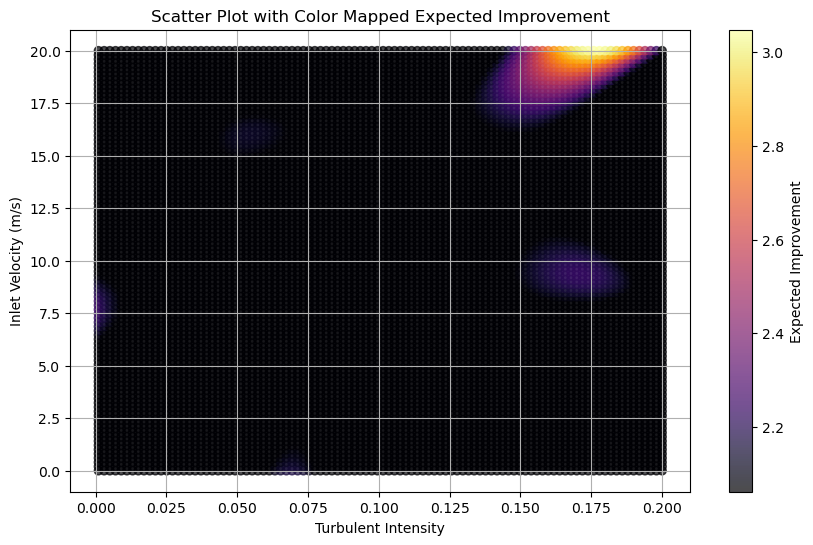
\includegraphics[width=\textwidth]{Images/ei_4.png}
            \caption[]%
            {{\small Optimisation 4}}    
            \label{fig:ei_4}
        \end{subfigure}
        \caption[]%
        {\small Expected Improvement Regions} 
        \label{fig:ei_optim}
\end{figure}

\clearpage

\begin{table}[ht]
\centering
\caption{Optimisation Steps}
\begin{tabular}{|l|ll|ll|}
\hline
\multicolumn{1}{|c|}{Sample} & \multicolumn{1}{c}{k} & \multicolumn{1}{c|}{U ($ms^{-1}$)} & \multicolumn{1}{c}{Recirc. Length (m)} & \multicolumn{1}{c|}{Ratio of H} \\ \hline
O1                           & 0.139697            & 15.959596                      & 0.375                                  & 1.875                           \\
O2                           & 0.161808           & 8.8888889                      & 0.36227                                & 1.81135                         \\
O3                           & 0.200000                  & 20.000000                               & 0.33133                                & 1.65665                         \\
O4                           & 0.179899            & 17.979798                      & 0.3467                                 & 1.7335                          \\ \hline
\end{tabular}
\label{tab:optim_values}
\end{table}


\section{Discussion}

From the plots of recirculation length in Fig.~\ref{fig:recirc_orig} and \ref{fig:recirc_optim}, it can be seen that the emulator was able to predict a range of values that mostly lie within the accepted values for the backwards facing step \cite{chen_review_2018}. The emulator was also able to demonstrate its ability to quantify the uncertainty in predictions through plots of standard deviation. In addition to this, the use of the acquisition function was successful at improving the quality of the overall model, shown through improvements in the recirculation length plot and in the reduction of the standard deviation.

From the plot of recirculation length resulting from the first 20 samples, shown in Fig.~\ref{fig:recirc_orig}, it can be seen that the emulator predicts a mostly linear 'ridge' of longer recirculation zones as the turbulent kinetic energy intensity and inlet velocity increase together. This falls in line with what would be expected, as the free stream velocity will drag the recirculation bubble out further. However, it could be argued that an increase in turbulent kinetic energy would result in the shear layer mixing faster with the recirculation bubble, resulting in a shorter reattachment length. This figure also has several parts that generate some questions and interest. Firstly, there is a darker (shorter) patch in the top half of the plot, and secondly, two of the corners have hit the colour map limit. The dark area is likely the model returning to the prior mean of 0, and this is corroborated by the higher standard deviation in this area shown in Fig.~\ref{fig:std_orig}. The expected improvement picks up on both of these metrics well, showing a clear region and peak for the next point to be evaluated in Fig.~\ref{fig:ei_orig}.

The optimisation steps shown in Fig.~\ref{fig:recirc_optim} demonstrate how the model changes with the addition of new and efficiently placed samples. The first optimisation step in Fig.~\ref{fig:recirc_1} shows a shrinkage of the dark patch and introduces changes along the bottom edge of the plot. This change does not carry over to the standard deviation plot which remains very similar in Fig.~\ref{fig:std_1}. However, examining the values on the colour bar, it can be seen that with each optimisation step, there is a reduction in the standard deviation values. With the 3rd and 4th optimisation steps, the standard deviation is lowered significantly across the whole plot, bar the bottom right corners. The high values seen in the bottom right corners of Fig.~\ref{fig:recirc_optim} represents a limitation of this implementation, where the true values are between 20-50. This shows the model does not have an understanding of the physical limits of the data it is representing, and in regions where the function carries on along the same gradient it left the last training point at. For this reason, it may be advisable to evaluate problems on a larger range than needed, and subsequently using just the inner portions of the models range where it is unaffected by a lack of samples near the edges. The lack of physical understanding may be remedied by the inclusion of prior knowledge which would likely reduce these issues, however this went beyond the scope of this project hence its exclusion.

From Fig.~\ref{fig:ei_optim}, it can easily be seen that the acquisition function was successful at choosing new spots to evaluate where the previous iteration had a low recirculation length as the model returned to a mean of 0 and where there was a higher standard deviation. In the context of CFD, where simulations are very time and energy intensive, the addition of this function represents a step in the efficiency of building an emulator when compared to purely stochastic sampling.

This model suffered due to the choice of the inlet velocity range, which meant that the majority of the sample space was operating in conditions that lend themselves to a stable recirculation area. This meant the model was attempting to predict very small changes in the wider sample space. To improve this project, instead of using inlet velocity as an input, a more appropriate choice would be the Reynolds number at the inlet. This would make the whole problem physically dimensionless and mean the flow characteristics could be easily controlled.


\section{Conclusion}
This paper has effectively reviewed and implemented surrogate modelling methods to build an emulator for the CFD analysis of the backwards facing step flow problem. This utilised state-of-the-art methods implemented via the toolbox \texttt{sciKitLearn} to map the input to output. There were also learnings into the efficient implementation of these methods, which were mainly around the generation and handling of raw data to ensure the model has the best chance of predicting correct and accurate results. This paper also demonstrated the power of active optimisation via use of acquisition functions, showing a decrease in the standard deviation of the model and an improvement in the overall model.

This project was also a successful group project, with all members contributing equally to the project. For the literature review and data gathering, the workload was split evenly and each member completed their work in a timely manner and to a high standard. For the implementation, the group all brought different parts to the table, resulting in a well applied end result.


\clearpage
\printbibliography

\appendix{Code Implementation}

\lstinputlisting[language=Python, caption= Latin Hypercube Sampler Code]{LHS.py}

\lstinputlisting[language=Python, caption= Emulator Code]{data_surrogate_script.py}

\clearpage


\end{document}
